% paper.tex
% sample ACM SIG Proceedings document using LaTeX2e
% Author: Heila van der Merwe
% based upon LaTeX2.09 Guidelines, 9 June 1996
% Revisions:  17 July 2012
%
\documentclass{acm_proc_article-sp}
\begin{document}


\title{Verifying Android Applications using Java PathFinder}

\numberofauthors{3}

\author{%
\alignauthor Heila van der Merwe\\
       \affaddr{Dept. of Computer Science}\\
       \affaddr{University of Stellenbosch}\\
       \affaddr{Private Bag X1 Matieland}\\
       \affaddr{South Africa, 7602}
       \email{hvdmerwe@cs.sun.ac.za}
\alignauthor  Brink van der Merwe\\
 \affaddr{Dept. of Computer Science}\\
       \affaddr{University of Stellenbosch}\\
       \affaddr{Private Bag X1 Matieland}\\
       \affaddr{South Africa, 7602}
       \email{abvdm@cs.sun.ac.za}
\alignauthor  Willem Visser\\
 \affaddr{Dept. of Computer Science}\\
       \affaddr{University of Stellenbosch}\\
       \affaddr{Private Bag X1 Matieland}\\
       \affaddr{South Africa, 7602}
       \email{wvisser@cs.sun.ac.za}
}

\maketitle

\begin{abstract}
Mobile application testing is a specialised and complex field. Due to mobile applications' event driven design and mobile runtime
environment, there currently exist only a small number of tools to verify these applications.

This paper describes the development of JPF-ANDROID, an Android application verification tool. JPF-ANDROID is built on Java PathFinder, 
a Java model checking engine. JPF-ANDROID provides a simplified model of the Android framework on which an Android application can run. It then allows
the user to script input events to drive the application flow. JPF-ANDROID provides a way to detect common property violations such as deadlocks and runtime exceptions
in Android applications.
\end{abstract}

\category{D.2.5}{Software Engineering}{Testing and Debugging}[Testing tools]

\terms{VERIFICATION}

\keywords{Mobile Application, Java PathFinder, JPF, Android, Verification, Testing}

\section{Introduction}
Software testing and verification plays an important role in determining the quality and robustness of software. These are two very
important attributes of mobile applications. Especially since users currently have more than 600 000 applications to choose from on the
Google Play Market.

Although software testing is so important, it is often neglected due to its complex and time consuming process. Android
applications face additional challenges when it comes to application testing. Firstly, they have an event based design which means that
their application flow is driven by graphical user interface (GUI) and system events. Secondly, Android applications are developed in a
custom implementation of the Java Application Programming Interface (API)  adopted from the Apache Harmony~\cite{harmony} project. The
compiled applications can only be executed on a special virtual machine (VM) called the Dalvik VM that runs on Android
devices~\cite{dalvik}.

Due to these challenges, the rapid pace at which mobile applications are developed and the lack of testing tools available, mobile
application testing is often omitted altogether. The simplest way to test GUI applications is manual black-box testing.
But, this is a time consuming, error prone and expensive~\cite{AccessibilityTech} process. One way to reduce this high cost, is to  automate
the testing of GUI -- in this case Android -- applications~\cite{AccessibilityTech}.

The most common way to automate Android application testing is to run tests on the Dalvik VM on a
physical device/emulator. Testing frameworks such as the MonkeyRunner and Robotium make use of Android's built-in JUnit
framework~\cite{TestingAndroid} to run test suites on the device. Running tests on the Dalvik VM is slow as they have to be instrumented and
each test sequence has to be defined and executed sequentially. Other projects use alternative ways to automatically generate input by
manipulating the built in accessibility technologies~\cite{AccessibilityTech} or by re-implementing the Android
keyboard~\cite{KeyboardModel}. Mockito and Android Mock allow JUnit testing on the Dalvik VM by using mock Android classes. The advantage of
testing applications on the Dalvik VM is that we can physically emulate input events on the device. The disadvantage is that it is not
simple to automate this input emulation. 

Another approach is to test Android applications using the Java Virtual Machine (JVM). There are different ways of implementing such
a framework. Android lint~\cite{lint}, for example, makes use of static analysis to identify common errors in applications.
Robolectric~\cite{robolectric}, a JUnit testing framework running on the JVM,  intercepts the loading of Android classes and then uses
shadows classes that model these classes.

Although Android applications and Java desktop applications are designed for completely different Java VMs, they are both built on an
implementation of the Java API. As a consequence, Android applications contain many of the same error as Java applications. These defects
include, but are not limited to, concurrency issues and common runtime exceptions such as NullPointer Exceptions. It follows that existing
Java testing frameworks can be adapted to verify Android applications.

% what are we going to do and why 
This paper describes an extension to Java PathFinder (JPF)~\cite{JPFDocs} that enables the automatic verification of Android applications on
the standard Java JVM. 

The next section will provide an overview of JPF and Android and how JPF can be used to test Android applications. Thereafter
the development of the JPF-ANDROID tool will be discussed. 

\section{Design}
\subsection{Java PathFinder}
JPF is an automated, open source, analysis engine for Java applications~\cite{JPFDocs}. It is implemented as an explicit state model checker
that includes mechanisms to model Java classes and native method calls (Model Java Interface - MJI Environment), track byte code execution
and listen for property violations. Additionally, JPF's design encourages developers to create extensions to the framework. Currently there
exist many extensions including a symbolic execution extension (JPF-SYMBC)~\cite{JPF-SYMB}, data race
detector (JPF-RACEFINDER) and an abstract window toolkit (AWT) extension (JPF-AWT)~\cite{JPF-AWT}.

JPF-AWT allows the model checking of AWT applications. AWT applications are event driven and based on a single
threaded, message queue design. All application events are put in a message queue and then handled by the main thread of the application,
called the EventDispatchThread. JPF-AWT introduced the idea of using a simple event script file to write sequences of user inputs to drive
the application execution. JPF-AWT models the EventDispatchThread so that when the message queue is empty, it requests an event from the
script file simulating the event occurring. 

JPF-ANDROID makes use of JPF's extension mechanisms to model the Android application framework so that Android applications can run on the
JVM. It then extends JPF-AWT's input model to simulate user and system input to drive the application flow. One of the advantages of
extending JPF is that it has been rigorously tested and can successfully detect many common defects in Java applications. As soon as Android
applications can run on JPF-ANDROID, common software errors are automatically detected.


\subsection{Android}
Android is an open source software stack for devices with an advanced RISC Machine (ARM) architecture.
It consists of the Android operating system (OS), the application framework and an application development toolkit assisting developers to create
applications for the platform~\cite{AndroidDocs}.

As shown in figure 1, the Android OS is built on top of a modified Linux kernel. The kernel provides a layer of abstraction on top of its
low level functionality such as process, memory, user, network and thread management. On top of the Android kernel is a set of native
C-libraries. The Dalvik VM is a custom, optimised version of the JVM. For security reasons each Android application is run as a separate
process in its own Dalvik VM instance~\cite{AndroidSecurity}.  Hence, applications can only communicate with each other and the with the
Android framework using Android's Binder inter-process communication (IPC) mechanism~\cite{Binder}. 

\begin{figure}
\centering
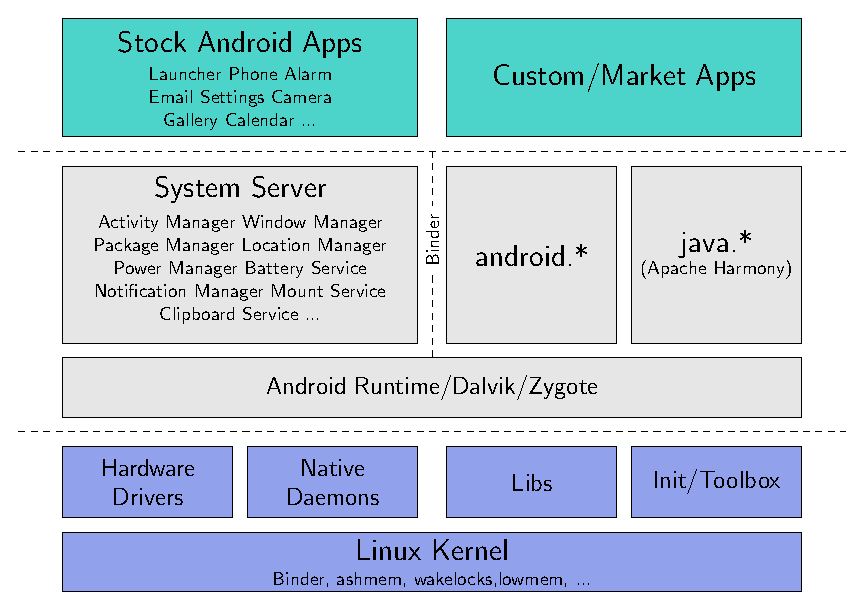
\epsfig{file=Stack.eps, width=3in,}
\caption{The Android application stack~\cite{systemserver}}
\end{figure}

Android has one main application called the system process. The system process contains services responsible for performing the main
tasks of the system including:
\begin{description}
 \item [ActivityManager] manages the life-cycle and interaction of all the activities running on the system
 \item [WindowManager] allows applications to draw on the screen and forwards UI input to the application.
 \item [PackageManager] stores information on the application packages installed on the device
\end{description}

All Android applications follow a single-threaded design in which the main thread of the application handles all application
events~\cite{AndroidDocs}. This structure is commonly used by many UI frameworks since it becomes too complex to make all UI classes thread
safe~\cite{SingleThread}. In Android, this main thread is called the \texttt{Looper} thread. The \texttt{Looper} has a message queue
attached to it containing all application events to be dispatched. UI and system events are scheduled on the main \texttt{Looper} by adding
them to the message queue. The \texttt{Looper} is responsible for continuously looping through these messages and handling them
appropriately. This could include updating a widget, loading a new activity or processing an Intent.

The main entry-point of each Android application is in its \texttt{ActivityThread} class. The \texttt{ActivityThread} class is part of the
Android framework and starts the application's \texttt{Looper} thread. It also keeps track of the application's components and handles user
and system events. Android applications also consists of the following application components:
\begin{description}
\item [Activity] responsible for representing and managing an user interface. An application can consist of many
Activities.
\item [Service] performs background operations such as the pulling of messages from a server every 5 minutes. Services do not have user
interfaces and an application can have zero or more services running simultaneously.
\item [Broadcast receiver] listens for and responds to system-wide events such as network failing, low battery or screen orientation
change events.
\item [Content provider] manages application data stored on the file system, in databases, on the web or other storage medium and provides a
gateway to this data from other applications.
\end{description}

These components interact with each other and with other applications using a structure called an \texttt{Intent}. An \texttt{Intent} is a
high level implementation of the Binder IPC.

\subsection{Scope of JPF-ANDROID}
The objective of JPF-ANDROID is to verify Android applications by running the application code on the JVM using a collection of different
event sequences and then to detect when certain errors occur using JPF.
%what scope of android will be modeled

The Android framework is very large and one of the main challenges of JPF-ANDROID is to decide which parts of the system to model. The more
of the Android framework is modelled, the more realistic the model is and the more errors can be found. But, if too much
of the framework is modelled the scheduling possibilities increase exponentially which means that the search space can become too big to
verify.

JPF-ANDROID focuses on verifying a single application with multiple application components and their interaction. The system service of
the Android OS is not part of the application process and runs in its own thread. To reduce scheduling possibilities, the entire system
service is not modelled but its necessary components are implemented as part of the application process. The following parts of the Android
framework is modelled:
\begin{description}
 \item [ActivityManager]  manages the life-cycle of Activities and other application components.
 \item [ActivityThread]   the main entry-point to the application. It controls and manages the application components and their input.
 \item [Application components] including Activity, Service, Broadcast Receiver and Content Provider. 
 \item [Window and View structure] The view hierarchy is modelled including the widgets and the window classes.
 \item [Message queue] modelled to support input from the script file.
\end{description}

Lastly, as the application will not be communicating with outside processes, the \texttt{Intent} objects are modelled to exclude the
Binder IPC service.

\section{Development}
\subsection{JPF-ANDROID architecture}
\begin{figure}
\centering
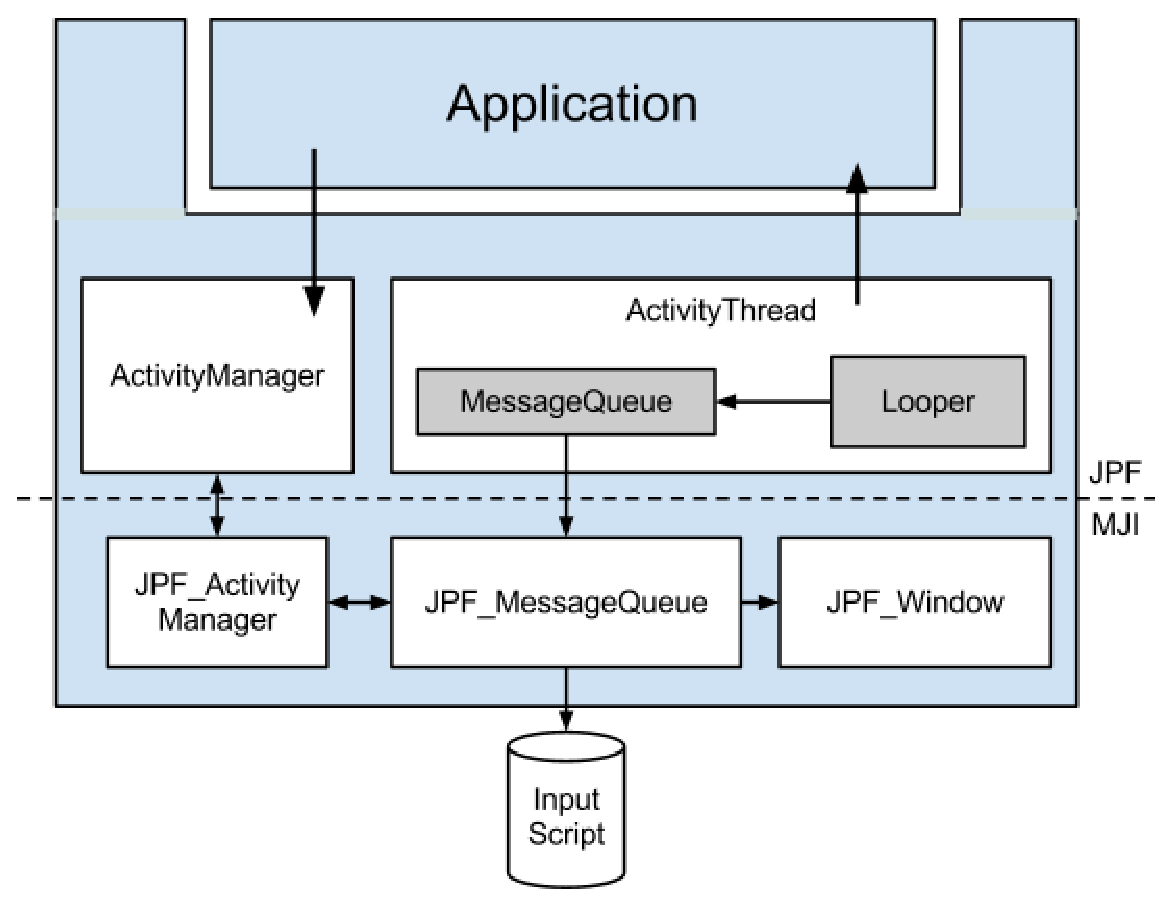
\epsfig{file=arch.eps, width=3.5in,}
\caption{JPF-ANDROID architecture}
\end{figure}
As discussed above, Android and AWT applications have a single-threaded application design. That is why JPF-ANDROID's architecture
is based on JPF-AWT. Figure 2 shows JPF-ANDROID's architecture. JPF-ANDROID models Android's message queue structure
by using JPF's MJI environment. When the \texttt{Looper} thread requests a new message from the message queue and it is empty, a call to the
native \texttt{JPF\_MessageQueue} class reads the next event from the input script file.

Android applications can receive input from two different sources: user input and system input. The
\texttt{JPF\_MessageQueue} class classifies events as either UI or system events. UI events are directed to and handled by the native
\texttt{JPF\_Window} class and system events are handled by the \texttt{ActivityManager} implemented as the
native \texttt{JPF\_ActivityManager} class.

When an Activity's UI (window) is inflated, an object map is created in the native \texttt{JPF\_Window} class. This
map binds the name of each widget to the reference of the inflated widget object. When an UI event is received by the native
\texttt{JPF\_Window} class, the name of the target widget is looked-up in the object map and the action is then called directly on the
inflated widget object by pushing a direct call frame on the JPF call stack. 

System events are a little more complex. They use \texttt{Intent} objects to describe a system event. \texttt{Intents} are used to start
Activities and Services or to provide a notification of certain events. They are similar to messages containing a description of an
operation to be performed or, often in the case of broadcasts, a description of something that has happened and is being
announced~\cite{AndroidDocs}. System events are handled by the native \texttt{JPF\_ActivityManager} class. This class keeps a map of Intents
as they are created in the script file. When a system event is received, the \texttt{ActivityManager} looks up the corresponding
\texttt{Intent} in the map. It then resolves the \texttt{Intent} to the relevant application and sends it to the application's
\texttt{ActivityThread} to be handled. This message will be processed by the \texttt{Looper} which will direct the \texttt{Intent} to the
corresponding application component.

\subsection{The input script}
AWT applications that are tested with JPF-AWT contains at least one input script. This script consist of a list of UI events. These
events are executed one-by-one when the message queue it empty. JPF-AWT's syntax only supports the scripting of UI events. To
allow users to script system events, variables were added to the scripting language. Variable names are identified by the ``@'' in front of
the name as '\$' is already used in JPF-AWT to identify UI components. These variable can be used to construct most Intent objects. For
example, a script file that sends an \texttt{Intent} to start the \texttt{SampleActivity} will contain:

{\small
{\sf
\hspace*{4mm}@intent1.setComponent(``com.example.SampleActivity'')\\
\hspace*{4mm}startActivity(@intent1)\\
\hspace*{4mm}\$button1.onClick()
}
}

JPF-ANDROID scripts also adopted the REPEAT and ANY constructs from JPF-AWT. REPEAT constructs repeat a list of events a specified number
of times. ANY constructs take a list of events and then uses a ChoiceGenerator and JPF's state matching and backtracking features to visit
each of the execution branches. JPF stores the state of the system before the it advances to a new state. JPF-AWT uses a JPF search listener
to store and retrieve the current position of the input script in a specific state so that the script's state is also saved.

Android applications contain multiple windows - one for each Activity. This complicates the script input as each window has its own unique
set of view components, hence, a unique input sequence. Furthermore, the application flow can switch between these Activities
at any point of execution. In other words, if we do not know in what Activity the application is, we can not schedule
the following events.

\begin{figure}
\centering
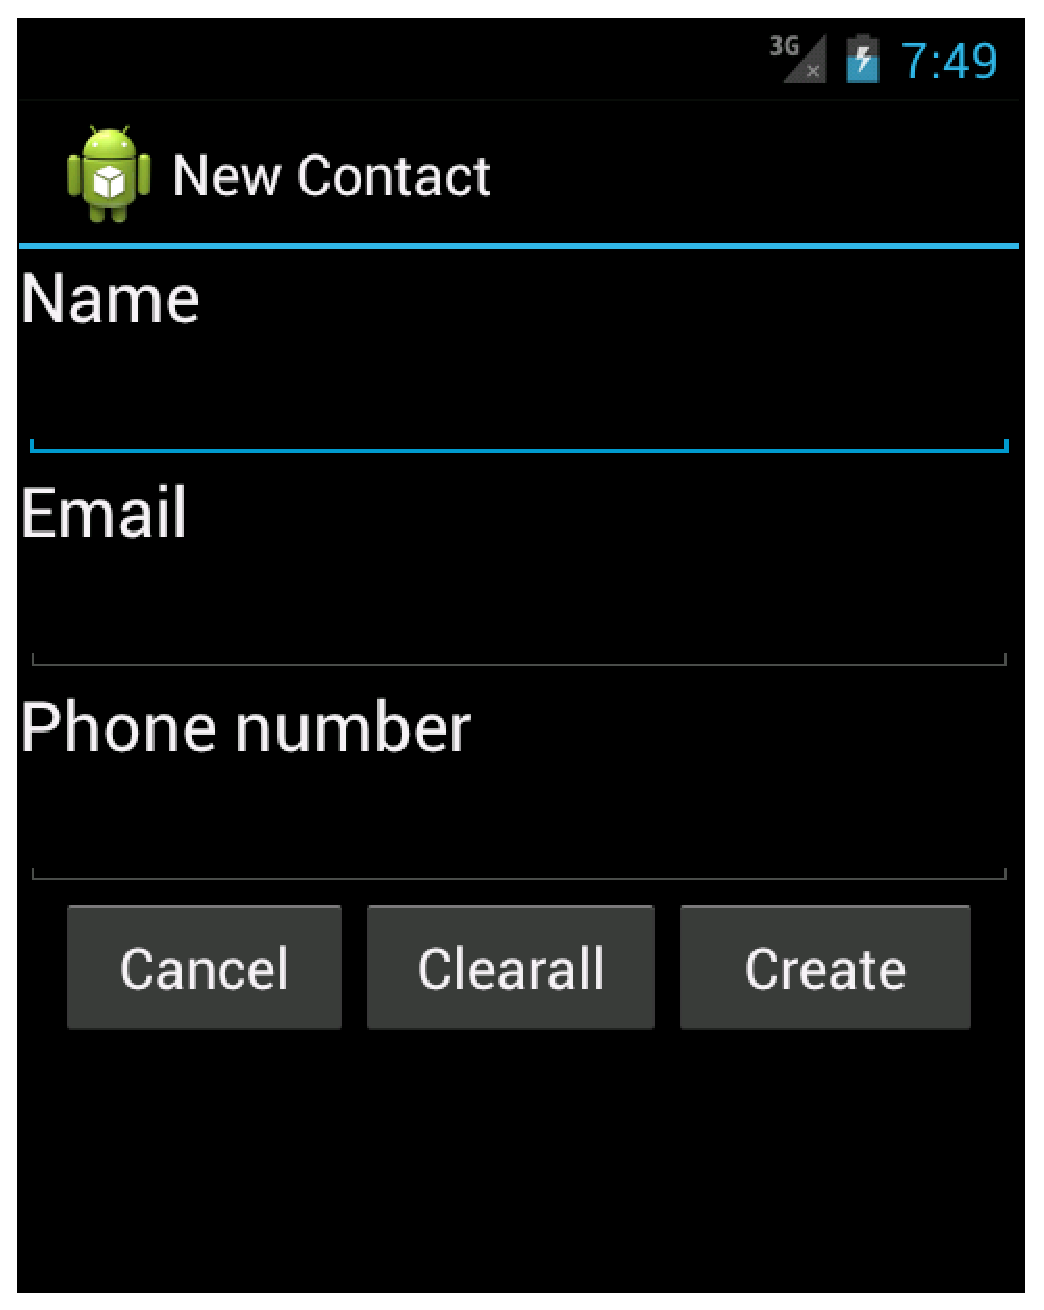
\epsfig{file=newContact.eps, width=1in,}\\
\caption{Contacts application window}
\end{figure}
\begin{figure}
{\small
{\sf
...\\
\textbf{ANY} \{ \$cancelButton.onclick(), \$clearButton.onClick()  \}
\$nameEdit.setText(``Mary'')\\
\$createButton.onClick()\\
...
}
}
\caption{Input script for ``New Contact'' window}
\end{figure}
Figure 3 displays the ``New Contact'' window of a Contacts application. It contains three
buttons: the cancel button restarts the \texttt{ListContactsActivity}, the clear button stays on the current Activity and the create 
button starts the \texttt{ViewContactActivity}. Now let us look at figure 4 containing the input sequence for the ``New Contact'' window.

The problem occurs in the ANY structure. When the cancelButton.onclick() event fires the application changes to another
Activity and the following events are not valid any more. To address this issue, we included the
use of sections in the input script (see figure 5). Each section groups the input events of a specific Activity. Now, if the cancel button
is pressed the \texttt{ListContactsActivity} will be started and then \texttt{ListContactsActivity}'s event sequence
will execute instead of executing the following events.

\begin{figure}
{\small
{\sf 
\textbf{SECTION} default \{\\
\hspace*{5mm}@startIntent.setComponent(``com.example.ListContactsActivity'')\\
\hspace*{5mm}startActivity(@startIntent)\\
\}

\textbf{SECTION} com.example.ListContactsActivity \{\\
\hspace*{5mm}\$createButton.onClick()\\
\hspace*{5mm}\$list.setSelectedIndex([0-3])\\
\}\\

\textbf{SECTION} com.example.AddContactActivity \{\\
\hspace*{5mm}\textbf{ANY} \{ \$cancelButton.onclick(), \$clearButton.onClick()  \}
\hspace*{5mm}\$nameEdit.setText(``Mary'')\\
\hspace*{5mm}\$createButton.onClick()\\
\}
}
}
\caption{Adding sections to the input script}
\end{figure}

Now lets view an Android application as a graph with each Activity as its nodes. The root of the tree is the applications main Activity. The
next challenge is to avoid an infinite loops in the application flow. If we look at the input in figure 5, an infinite loop will occur. The
ListContactsActivity starts the AddContactActivity and when the cancel button is pressed the AddContactActivity returns to
the ListContactsActivity. To solve this problem, JPF-ANDROID stores its current Activity. When input events are requensted by the input
script they are read from the current Activity's script section. The current position in this script file is also stored. When the
application forwards to a next activity, the state of all the visited activities in the execution path is stored. So when JPF backtracks
the the state of previous Activity's script files are continued instead of restarted. So when AddContactActivity returns to
ListContactsActivity, the script is not restarted but continued.

\subsection{Case study}

Currently JPF-ANDROID can detect deadlocks, race conditions and other property violations in Android applications. The challenge is
providing a sample application to show how JPF-ANDROID works. This is because most Android applications make use of Android specific
libraries such as a sqlite database connector, HTTP connection or the mediaplayer libraries. The future work of JPF-ANDROID
includes modelling these Android specific libraries.

To show how JPF-ANDROID works, we will use a calculator application.






\section{Conclusion}
The paper discussed the design and implementation of JPF-ANDROID. JPF-ANDROID is still under development and currently only models
the core libraries needed to verify a basic Android application. It allows Android applications to be tested using JPF's proven verification
techniques and can successfully detect common Java errors such as runtime exceptions and deadlocks. 

This extension provides a basis on which Android applications can be tested. It can later be extended to verify functional requirements
and identify Android specific errors using JPF's listener mechanism.

Future extensions include modelling a sqlite database and http connections.

%
% The following two commands are all you need in the
% initial runs of your .tex file to
% produce the bibliography for the citations in your paper.
\bibliographystyle{abbrv}
\bibliography{paper}  % sigproc.bib is the name of the Bibliography in this case

\end{document}
